\section{Reinforcement learning (RL)}~\label{ssec:rl}
\noindent Please note that this is an aggressively shortened summary. For a deeper introduction please refer to \cite{SB_all}.
The Reinforcement learning problem originates from the idea of learning by interacting with an environment. The object that is learning is doing so by retrieving information from cause and effect. The causal model that is learned in such a way is updated with each change of the environment that can be related to some action. Therefore the learned model fits the true model increasingly better with the number of induced causes and observed effects.\\
This type of learning problem can be modeled by "Finite Markov Decision Processes". Such a model usually needs the following elements:\\

\begin{itemize}
	\item \textbf{Environment}\\
	The environment is an object inheriting one ore multiple complex physical processes. Information on the current state of that process are typically obtained by measurements in the physical environment itself or by evaluating a computer model of the actual environment.
	\item \textbf{State}\\
	The state $s_t$ is generated by the environment and reflects the current state that the environment is in. It changes over time according to the dynamics within the environment.
	\item \textbf{Action}\\
	An action $a_t$ is a cause that might change the state of the environment. Actions are produced by the agent.
	\item \textbf{Reward} The reward $r_t$ is a scalar value that is produced by the environment and received by an agent.
	\item \textbf{Agent}\\
	The agent is an object which generates actions $a_t$ and observes the caused change from $s_{t-1}$ to $s_t$ of the environment as well the along going reward $r_t$.
	\item \textbf{Policy}\\
	A policy $\pi(a_t|s_t)$ is a probability distribution over the set of possible actions $a_t$ given the state $s_t$ at a time step $t$. A agent is essentially defined by its policy as each action that is taken is sampled from that policy.
\end{itemize}

The signal flows between agent and environment are depicted in figure \ref{fig_rl_gen}

\begin{figure}
	\centering
	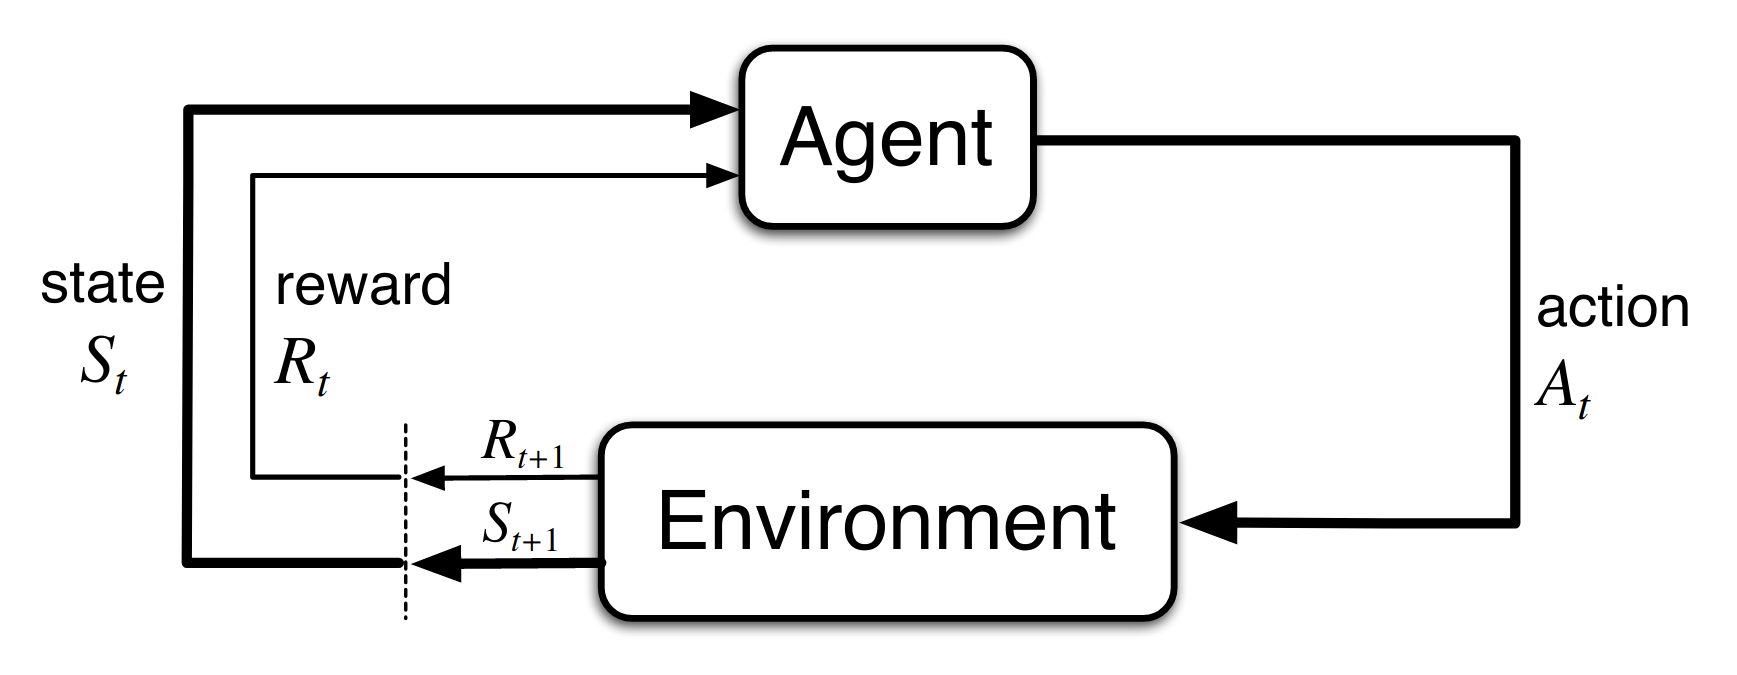
\includegraphics[width=0.8\textwidth]{figures/rl/agent_env_interface}
	\caption{agent environment interaction \cite{SB_all}}
	\label{fig_rl_gen}
\end{figure}

All signals in this model are time dependent. 
Such a model satisfies the Markov Property if the next state $s'$ and reward $r$ only depend on the current state action tuple $(s, a)$. If assuming finite state and action spaces together with the Markov property yields a Finite Markov Decision Process. The environment dynamics can therefore be represented by the bi-variate probability distribution
\begin{align}
	p(s', r|s, a) = Pr\{r_{t+1}=r, s_{t+1} = s' | s_t=s, a_t=a\}
\end{align}
Further, if $a_t$ is sampled from $\pi(a_t|s_t)$ the Markov Property induces conditional independence of $(s_{t-1}, r_{t-1})$ and $(s_{t+1}, r_{t+1})$ given $s_t$. \\

The agents task is to predict a policy that maximizes the expected future rewards. This objective is given by
\begin{align}
	\argmax_{\pi}\mathop{\mathbb{E}}_{p_{\pi}}\left[\sum_{t=0}^T r_t | s_0\right]
\end{align}
Here $T$ marks the time limit of the process and $p_{\pi}$ represents the environment dynamics following a action history sampled from $\pi$.\\

\subsection{Value functions}
Most methods aiming to solve eq. (2.2) use estimations of so called value functions. This are functions that provide a quality measure for an agent evaluating a state or a state action tuple. \\
Commonly three value functions are used. The state value function, the state action value function and the advantage value function.\\
They all depend on the expected discounted future rewards
\begin{align}
	g_t = \sum^{T-t-1}_{k=0} \gamma^k r_{t+k+1} .
\end{align}
Here $\gamma$ is referred to as the discount factor. Its value usually determines how prospective future rewards are weighted in the value function. E.g if $\gamma<1$ rewards that are closer to $t$ get a higher weight than those that are occuring at later time steps. For $\gamma>1$ the contrary holds.\\
The state value function is defined by
\begin{align}
	V_{\pi}(s) = \mathop{\mathbb{E}}_{p_{\pi}}\left[g_t|s_t=s \right]\text{,}
\end{align}
the state action value by
\begin{align}
	Q_{\pi}(s, a) = \mathop{\mathbb{E}}_{p_{\pi}}\left[g_t|s_t=s, a_t=a \right]
\end{align}
and finally the advantage value by
\begin{align}
	A_{\pi}(s, a) = Q_{\pi}(s, a) - V_{\pi}(s)
\end{align}
it follows
\begin{align}
	V_{\pi}(s) = \mathop{\mathbb{E}}_{a\sim\pi}\left[ Q_{\pi}(s, a)\right]
\end{align}

\noindent Usually the objective is to maximize either one or more value functions.
Note that, $\max_{\pi}V_{\pi}(s)$ and $\max_{\pi}Q_{\pi}(s, a)$ satisfy Bellman's principle of optimality. Hence they can be solved exactly with Dynamic Programming. This is referred to as the tabular solution. However for most problems this is not feasible and the value functions are approximated by neural networks. \\

\subsection{Q-learning}
Q-learning is a method to find the state action value maximizing policy by minimizing temporal differences. This is often the backbone for policy gradient algorithms. Let
\begin{align}
\pi(a|s) = \delta(a - \argmax_{a'}Q_{\pi}(s, a'))
\end{align}

where $\delta$ is the Dirac delta function. Therefore sampling from the policy yields the maximum action state value. The objective is to approximate $Q_{\pi}$ which is achieved by the temporal difference loss
\begin{align}
\mathcal{L}_{TD} = \frac{1}{2} \left(r_{t} + \gamma \max_{a}Q_{\pi}(s_{t+1}, a) - Q_{\pi}(s_t, a_t)\right)^2.
\end{align}
this kind of approximation is usually referred to as one step temporal difference method. The optimality follows directly and the convergence of the approximation under certain conditions has been proven in \cite{SBQL}.\\
In contrast to one step temporal difference methods there are Monte Carlo methods which collect the loss over whole episodes. One episode is defined by the history of temporal differences between the starting state $t=0$ and an end state $t=T$. This methods usually use eligibility traces \cite{SBeligibility}. \\
Optimizing eq. (2.9) is referred to as on-policy policy optimization where the target policy $\pi$ is the policy which is used when actions are sampled. This however is problematic as the target policy, defined by eq. (2.8) depends on $Q_{\pi}$ which is not trustworthy in early training iterations as this is the approximating function. In order to have more control over the sampling of actions which is usually referred to as exploration, a data collection policy $\mu(a|s)$ is used during training. Therefore in an off-policy setting, eq. (2.9) is redefined to
\begin{align}
\mathcal{L}_{TD} = \frac{1}{2} \left(r_{t} + \gamma \max_{a}Q_{\mu}(s_{t+1}, a) - Q_{\mu}(s_t, a_t)\right)^2\text{.}
\end{align}
and during inference 
\begin{align}
\bar{\pi}(a|s) = \delta(a - \argmax_{a'}Q_{\mu}(s, a'))
\end{align}
is used. Off policy methods fight the issue of the distributional mismatch between the target policy $\pi$ and the exploration policy $\mu$. There are many solutions to overcome this mismatch. Many use importance sampling or variance reduction techniques.\cite{liu2018breaking}

\subsection{Policy gradient methods}

This class of algorithms optimize the parameters $\theta$ of a policy $\pi_\theta(a|s)$. Let 
\begin{align}
\rho(\pi) = \sum_{t=1}^{\infty}\mathop{\mathbb{E}}_{\substack{s\sim d_\pi(s) \\ a\sim \pi(a|s)}} \left[ r_t|s_0 \right] = V_\pi(s_0)
\end{align}
be the expected, discounted future reward per step and let
\begin{align}
d_\pi(s) = \sum_{t=0}^\infty \gamma^t Pr\left\{s_t=s|s_0, \pi\right\}
\end{align}
be the discounted stationary distribution of states under $\pi$. Then
\begin{align}
\frac{\partial\rho_\pi}{\partial\theta} = \sum_s d_\pi(s)\sum_a \frac{\partial\pi(a|s)}{\partial\theta} \bar{Q}_\pi(s,a)
\end{align}
Is the policy gradient with which gradient ascent on the policy can be performed in order to maximize $\rho$. A proof and a thorough discussion can be found in \cite{PGBS}. Note that the policy gradient is on-policy and that $\bar{Q}_\pi$ is an approximation of the exact state action value function $Q_\pi$.\\
Since $\pi$ is a probability distribution it follows that $\sum_a\frac{\partial\pi(a|s)}{\partial\theta}=0, \forall s \in S$. Eq. (2.14) can therefore be rewritten as
\begin{align}
\frac{\partial\rho_\pi}{\partial\theta} = \sum_s d_\pi(s)\sum_a \frac{\partial\pi(a|s)}{\partial\theta}\left[ \bar{Q}_\pi(s,a)+b(s)\right],\text{\hspace{12mm}} b:S\rightarrow \mathop{\mathbb{R}}.
\end{align}
The function $b$ is called a baseline and is often used to reduce variance and bias in the gradient. Using $\frac{\nabla_\theta\pi(a|s)}{\pi(a|s)} = \nabla_\theta ln(\pi(a|s))$ and $\mathop{\mathbb{E}}_{x\sim p(x)}[f(x)] = \sum_{x}p(x)f(x)$, rewriting eq (1.13) yields
\begin{align}
\frac{\partial\rho_\pi}{\partial\theta} = \mathop{\mathbb{E}}_{\substack{s\sim d_\pi(s) \\ a\sim \pi(a|s)}}\left[ \nabla_\theta ln (\pi(a|s))\left[ \bar{Q}_\pi(s,a)+b(s)\right]\right].
\end{align}
In practice there are large state and action spaces, thus the expectations w.r.t $s$ and $a$ become infeasible to obtain. Using $\mathop{\mathbb{E}}_{x\sim p(x)}[f(x)] = \frac{1}{n}\sum_{n}f(x), n\rightarrow\infty, x\sim p(x)$ , sample based learning uses enough samples of $s$ and $a$ in order to obtain a good enough approximation of the expectations. Therefore the approximation of eq. (2.16) is

\begin{align}
\frac{\partial\rho_\pi}{\partial\theta} \simeq \frac{1}{n}\sum_{n} \nabla_\theta ln (\pi(a|s))\left( \bar{Q}_\pi(s,a)+b(s)\right),\text{\hspace{8mm}} s\sim d_\pi(s), \text{\hspace{4mm}} a\sim \pi(a|s), \text{\hspace{4mm}} n\rightarrow N
\end{align}
Here $N$ is the number of samples drawn which is in practice usually $N=1$.
This leads to Actor Critic methods where there are two instances that are updated in a turn based fashion. The critic is the state action value function approximation and the actor is approximating the policy with the policy gradient. Intuitively the critic evaluates the action taken by the actor who uses this evaluation to scale its gradient update (this is the role of $\bar{Q}_\pi$ in eq. (2.17)).

\subsection{Maximum Entropy Reinforcement Learning}
In off-policy settings it is common to use a data collection policy $\mu$ which has a large entropy in order to encourage exploration of the action and state spaces. The principle of maximum causal entropy has been introduced by \cite{AAAIziebert} and was elaborated on, among others, by \cite{DBLP:journals/corr/HaarnojaTAL17}. The key idea is to incorporate an entropy term into the objective function, acting like a regularizer. 

\begin{align}
\rho^{\mathcal{H}}(\pi) = \sum_{t=1}^{\infty}\mathop{\mathbb{E}}_{\substack{s_t \sim d_\pi(s_t) \\ a_t \sim \pi(a_t|s_t)}} \left[ r_t + \alpha(t) \mathcal{H}(\pi(\cdot | s_t))|s_0 \right]
\end{align}
Here $\alpha$ is a non-negative regularization weight which is usually monotonically decreasing with increasing $t$ and $\mathcal{H}$ is some entropy measure. If $\alpha$ becomes $0$, eq. (2.18) is equal to eq. (2.12), therefore intuitively $\alpha$ should be high in the early phase of training the policy and value function and converge to $0$ as the policy gets closer to the optimal policy.\\
This objective is on-policy and still gives control over the exploration behavior. Usually it does not bother if the policy has high entropy, since during inference the action where "\pi" has maximum probability is selected strictly. This makes especially unimodal distributions attractive. They fixate on single actions and they imply few parameters only that need to be learned (e.g. mean and variance of normal distributions). However often more expressive multimodal distributions fit the true distribution which is approximated better. 
In \cite{DBLP:journals/corr/abs-1906-02771} this idea has been extended by using  normalizing flows. Normalizing flows \cite{papamakarios2019normalizing} are based on the idea of transforming a probability density function by letting each sample undergo a transformation. If this transformation is a diffeomorphism, the probability of the transformed sample can be determined. Let $T$ be a diffeomorphism of a real vector $u$ sampled from $q(u)$.

\begin{align}
	x=T(u) \text{\hspace{5mm}where\hspace{5mm}} u\sim q(u)
\end{align}
then
\begin{align}
p(x)=q(T^{-1}(u)) |detJ_T(u)|^{-1}
\end{align}
where $J_T(u)$ is the Jacobian matrix of $T$ w.r.t. $u$. In practice, an invertible neural network can be trained to transform a simplistic density function into a more expressive one.\\
E.g. let the agent predict mean and variance of a Normal distribution. Then in the data collection process, actions are sampled from a transformed Normal distribution where the transform encourages entropy and maybe also multiple modes. Assuming the sampling happened using the reparametrization trick (see section \ref{ssec:reparam}), then the log probabilities and their gradient in eq (2.17) can still be calculated. This is a on-policy training with a expressive density function and the advantage is that easy reparameterization can still be used, as sampled is from the base distribution.

\subsection{Soft Actor-Critic (SAC)}\label{ssec:sac}
This algorithm was introduced by \cite{haarnoja2018soft}. They aim is to maximize the objective in eq. (2.18). Particularly they focus on the selection of the weight factor $\alpha$ and show, that it can be seen as a learnable parameter which is trained jointly with actor and critic networks.\\
The SAC is derived from the soft policy iteration where the temporal difference equation for the action value depends on the soft value function which is defined as
\begin{align}
	V_{\pi}(s_t) = \mathop{\mathbb{E}}_{a \sim \pi(a|s_t)} \left[ Q_{\pi}(s_t, a) - \alpha log( \pi(a|s_t)) \right].
\end{align}
Here the negative log probabilities correspond to the entropy measure $\mathcal{H}$ in eq. (2.18). The state action value function loss yields
\begin{align}
	\mathcal{L}_{critic} = \frac{1}{2}(Q_{\pi}(s_t, a_t) - (\gamma \mathop{\mathbb{E}}_{s_{t+1} \sim d_{\pi}(s)} \left[ V_{\pi}(s_{t+1})\right] + r_t)) ^ 2.
\end{align}

For the policy improvement step the policy is updated such that it approximates $\softmax_a(\frac{1}{\alpha}Q_{\pi}(s, a))$ where $Q_{\pi}$ is the soft action value function, learned by minimizing eq. (2.22). The loss for the policy then yields

\begin{align}
\mathcal{L}_{actor} = DKL_{a}\left[ \pi(a| s_t) \bigg|\bigg| \frac{exp(\frac{1}{\alpha} Q_{\pi}(s_t, a))}{Z(s_t)} \right].
\end{align}

Here $DKL_{a}$ is the Kullback Leibler Divergence over the actions and $Z(s_t)$ is the partition function in the softmax distribution. 

\begin{align}
	Z(s_t) = \sum_a Q_{\pi} (s_t, a)
\end{align}

It is usually too expensive to evaluate $Z(s_t)$ since it involves integrating/summing over the state action value space which means many forward passes through the neural network that represents $Q_{\pi}$. Since $\mathcal{L}_{actor}$ is minimized by gradient descent methods, only the gradient of eq. (2.23) is needed. If the KL-divergence term is expanded, $log(Z(s_t))$ becomes an additive term and therefore vanishes in the gradient.\\
Note that $\alpha$ in eq. (2.23) gives control over the differences between state action values and therefore over the entropy in the resulting softmax distributution. \emph{Lemma 2} in \cite{haarnoja2018soft} claims the improvement of $Q_{\pi}$ with each optimization step of $\mathcal{L}_{actor}$.\\
The gradient of eq. (2.23) w.r.t. the parameters $\theta$ of $\pi$ yields

\begin{align}
\nabla_\theta \mathcal{L}_{actor} = \nabla_\theta \mathop{\mathbb{E}}_{\substack{s_t \sim d_\pi(s_t) \\ a_t \sim \pi(a_t|s_t)}} \left[ \alpha log(\pi(a_t|s_t)) - Q_\pi(s_t, a_t) \right]
\end{align}

approximating eq. (2.24) by a sample based method yields

\begin{align}
\nabla_\theta \bar{\mathcal{L}}_{actor} = \nabla_\theta \left[ \alpha log(\pi(a_t|s_t)) - Q_\pi(s_t, a_t) \right]
\end{align}

minimizing this loss by a gradient descent method involves backpropagating the gradient through a sampling procedure. This can be made differentiable by the reparameterization trick (see section \ref{ssec:reparam}).\\
The authors in \cite{haarnoja2018soft} also provide a method to determine the entropy adjustment $\alpha$ such that it takes the minimal value needed to maximize the maximum entropy objective in eq. (2.18), assuming a fixed policy $\pi$.\\
In practice, reinforcement learning problems have high dimensional action spaces but only one dimensional rewards. Therefore the learned state action value function of the critic is also one dimensional in contrast to the actor who predicts the statistics for either the policy for each action dimension or the statistics for a multivariate probability distribution covering all actions. For the former the joint probability is the product of probabilities over all actions. This results in summing the log probabilities of the actions in eq. (2.26).

\subsection{Common optimization methods}\label{ssec:common_opt}
There are numerous optimization methods for reinforcement learning problems. This is just a listing of only very few but important ones, reviewed and evaluated in \cite{hessel2017rainbow}.

\begin{itemize}
	\item \textbf{Double Q-learning} \label{text:doublQ}\\
	Conventional Q-learning is affected by an overestimation bias of state action values. The authors in \cite{DBLP:journals/corr/HasseltGS15} decouple the action selection from its evaluation by learning two state action value functions independently resulting in the loss
	
	\begin{align}
		\mathcal{L}_{TD} = \frac{1}{2} \left(r_{t} + \gamma Q_{\pi}^{(\bar{\phi})} \left( s_{t+1}, \argmax_{a}Q_{\pi}^{(\phi)}(s_{t+1}, a) \right) - Q_{\pi}^{(\phi)}(s_t, a_t)\right)^2\text{.}
	\end{align}
	
	Here $\phi$ and $\bar{\phi}$ are the parameters of the independently trained state action value functions respectively. A similar method trains two action value functions independently and and takes for all evaluations the min value of the two network predictions. Both methods show a reduction in overestimation.
	
	\item \textbf{Prioritized replay}\\
	During data collection the tuples $(s_t, a_t, r_{t}, s_{t+1})$ are stored in a replay buffer. During training phases it is sampled uniformly from that buffer.\\
	In \cite{schaul2015prioritized} the sampling is not uniform but rather with a probability $p_t$ relative to the last encountered loss of that replay tuple.
	\begin{align}
		p_t \propto \mathcal{L}_{TD} ^ \omega \text{.}
	\end{align}
	Raising the loss to the power of the parameter $\omega$ determines the shape of the distribution. New transitions that did not produce a loss yet are always sampled with maximum priority.
	
	\item \textbf{Multi-step learning}\\
	Q-learning bootstraps from single step temporal difference losses. The authors in \cite{SBQL} introduced multi-step temporal differences which is the transition from Monte Carlo methods to single step temporal difference methods. The $n$-step return is defined as 
	
	\begin{align}
		r_t^{(n)} \equiv \sum_{k=0}^{n-1} \gamma_t^{k} r_{t+k+1}
	\end{align}
	
	then the multi step temporal difference loss yields,
	
	\begin{align}
		\mathcal{L}_{TD} = \frac{1}{2} \left(r_{t+1}^{(n)} + \gamma^{n} \max_{a}Q_{\pi}(s_{t+n}, a) - Q_{\pi}(s_t, a_t)\right)^2
	\end{align}
	
	optimizing multistep temporal difference losses with $n$ sampled uniformly from the interval $[1..T]$ results in faster learning.
	
	\item \textbf{Dueling networks}\\
	This was introduced by \cite{DBLP:journals/corr/WangFL15}. It is an optimization method based on the neural network atrchitecture of value functions in value based RL. It features one state-value and one advantage-value stream of computation that both share a common state feature extractor network $f(s)$. This leads to this factorization of action-values
	\begin{align}
		Q_{\pi}^{(\phi)}(s, a) = V_{\pi}^{(\eta)}(f^{(\xi)}(s)) + A_{\pi}^{(\psi)}(f^{(\xi)}(s), a) - \frac{\sum_{a'} A_{\pi}^{(\psi)}(f^{(\xi)}(s), a')}{N_{actions}}
	\end{align}
	
	Here $\eta, \psi$ and $\xi$ are the parameters of the state value function, the advantage value function and the state feature extractor respectively. $\phi$ is the concatenation of $\eta, \psi$ and $\xi$.\\
	The last term in eq. (2.31) approximates $\mathop{\mathbb{E}}_{a' \sim \pi} A_{\pi}^{(\psi)}(f^{(\xi)}(s), a')=0$. This equality follows from combining eq (2.6) and eq(2.7). Then eq. (2.31) follows from eq. (2.4), eq. (2.5) and eq. (2.6).\\
	This method outperforms value based RL methods on common RL benchmarks. 
	
	\item \textbf{Asynchronous Advantage Actor Critic (A3C)} \label{ssec::a3c}\\
	The authors in \cite{mnih2016asynchronous} define an asynchronous learning method for actor critics. Here multiple actors and critics optimize the same parameters of value function and policy in parallel based on a common replay buffer. Depending on how much memory and cpu/gpu cores are available this can speed up learning significantly.
	
\end{itemize}
